\documentclass[a4paper]{article}
% Import some useful packages
\usepackage[margin=0.5in]{geometry} % narrow margins
\usepackage[utf8]{inputenc}
\usepackage[english]{babel}
\usepackage{hyperref}
\usepackage{bm}
\usepackage{listings}
\usepackage{amsmath,graphicx,varioref,verbatim,amsfonts,geometry,amssymb,dsfont,blindtext,wasysym}
%\usepackage{minted}
\usepackage{amsmath}
\usepackage{xcolor}

\usepackage{placeins}

\let\Oldsection\section
\renewcommand{\section}{\FloatBarrier\Oldsection}

\let\Oldsubsection\subsection
\renewcommand{\subsection}{\FloatBarrier\Oldsubsection}

\let\Oldsubsubsection\subsubsection
\renewcommand{\subsubsection}{\FloatBarrier\Oldsubsubsection}

\hypersetup{colorlinks=true}
\definecolor{LightGray}{gray}{0.95}
\definecolor{dkgreen}{rgb}{0,0.6,0}
\definecolor{gray}{rgb}{0.5,0.5,0.5}
\definecolor{mauve}{rgb}{0.58,0,0.82}
\definecolor{mygray}{rgb}{0.9,0.9,0.9}
\definecolor{LightGray}{gray}{0.95}
\lstset{frame=tb,
	language=Python,
	aboveskip=3mm,
	belowskip=3mm,
	showstringspaces=false,
	columns=flexible,
	basicstyle={\small\ttfamily},
	numbers=none,
	numberstyle=\tiny\color{gray},
	keywordstyle=\color{blue},
	commentstyle=\color{dkgreen},
	stringstyle=\color{mauve},
	backgroundcolor=\color{mygray}
	%breaklines=true,
	%breakatwhitespace=true,
	%tabsize=3
}

\usepackage{enumitem}
\setlistdepth{20}
\renewlist{itemize}{itemize}{20}
\setlist[itemize]{label=$\cdot$}

\title{Project 4 in FYS3150}
\author{Bendik Steinsvåg Dalen}
%\renewcommand\thesection.\alph{section}
%\renewcommand\thesection{\Alph{section}}
\renewcommand\thesubsection{\thesection.\alph{subsection}}
\renewcommand\thesubsubsection{\thesubsection.\roman{subsubsection}}
\begin{document}
\maketitle


\section{ABSTRACT}

In this project we have studied the Ising model of a magnetic system using the Metropolis algorithm. We found that the steady state situation was often found within $10^5$ Monte-Carlo cycles, and that the critical temperature $T_C$ is around $T=2.3 J/k_B K$.

\section{INTRODUCTION}

The Ising model in two dimensions is a popular model for simulating phase transitions. The Ising model is a binary system, as in each object, or lattice site, can only have one of two values. At a certain critical temperature $T_C$ the model goes through a phase transition, from a phase with magnetization to a phase with zero magnetization. It is what occurs around this temperature we want to study. 

In this project we are going to test the Metropolis algorithm when applied to the Ising model. We want to test how many Monte-Carlo cycles are needed for the system to achieve a steady state situation, where the variance in each cycle is small. We are then going to use this to study how the system behaves close to the critical temperature. 

\section{METHOD}

\subsection{The Ising model}

The Ising model we will use consists of a $L\times L$ matrix $s$, with $N=L^2$ object. $L$ is also sometimes referred to as lattice. In our case each object is a spin $s_k$, that can be either $+1$ or $-1$. The energy of the Ising model is
\begin{align}
E = -J\sum_{<kl>}^{N}s_{k}s_{l}, \label{energy}
\end{align}
where $J$ is a coupling constant expressing the strength of the interaction between neighboring spins, and $<kl>$ means we sum over the nearest neighbors only. Essentially each spin will form a pair with the spins surrounding it. We then add up all the pairs, making sure to only count them once. We will also use periodic boundary conditions, meaning that the spins on the edge of the matrix can form pairs with the spins on the opposite side. 

In addition we know some analytical formulas describing the the Ising model; the partition function $Z$, and the corresponding expectations values for the energy $E$, the mean absolute value of the magnetization $|M|$, the specific heat $C_V$ and the susceptibility $\chi$. $Z$ can be found with
\begin{align}
Z &= \sum_{i=1}^{m} e^{-\beta E_i},
%= e^{8\beta J} + 4e^{0\beta J} + 4e^{0\beta J} + 2e^{-8\beta J} + 4e^{0\beta J} + e^{8\beta J} 
%= 2e^{8\beta J} + 2e^{-8\beta J} + 12 
\end{align}
where $i$ is a possible microstate for $s$, $E_i$ is the energy of that microstate, $m$ is all the microstates, and $\beta = 1/k_BT$. $k_B$ is the Boltzmann constant and $T$ is the temperature. The expectation value for $E$ can be found with
\begin{align}
\langle E \rangle = \frac{1}{Z} \sum_{i=1}^{m} E_i e^{-\beta E_i}.
%&= kT^2 \left( \frac{\partial \ln Z}{\partial T} \right)_{V,N} 
%= kT^2 \left( \frac{\partial }{\partial T} \ln \left[ 2e^{8\beta J} + 2e^{-8\beta J} + 12 \right]  \right)_{V,N} \\
%&= kT^2 \frac{1}{2e^{8\beta J} + 2e^{-8\beta J} + 12} \left(-\frac{2\cdot 8 \cdot J e^{8\beta J}}{kT^2} + \frac{2\cdot 8 \cdot J e^{- 8\beta J}}{kT^2} \right) 
%= \frac{8 J e^{- 8\beta J} - 8 J e^{8\beta J} }{e^{8\beta J} + e^{-8\beta J} + 6} 
\end{align}
The expectation value for $|M|$ is
\begin{align}
\langle |M| \rangle &= \frac{1}{Z} \sum_{i=1}^{m} M_i e^{-\beta E_i},
%= \dfrac{4 e^{8\beta J} + 2 \cdot 4e^{0\beta J} + 0\cdot 4e^{0\beta J} + 0\cdot 2e^{-8\beta J} + 2\cdot 4e^{0\beta J} + 4	\cdot e^{8\beta J} }{Z}\\
%&= \dfrac{8 e^{8\beta J} + 16}{2e^{8\beta J} + 2e^{-8\beta J} + 12}
%= \dfrac{4 e^{8\beta J} + 8}{e^{8\beta J} + e^{-8\beta J} + 6}
\end{align}
where $M_i$ is the magnetization at the microstate $i$. The specific heat can be found with
\begin{align}
C_V &= \frac{1}{k_BT^2} \left( \langle E^2 \rangle - \langle E \rangle ^2 \right)
= \frac{1}{k_BT^2} \left( \frac{1}{Z} \sum_{i=1}^{m} E_i^2 e^{-\beta E_i} - \langle E \rangle ^2 \right),
%&= 
%\frac{1}{k_BT^2} 
%\left( \frac{ (-8J)^2 \cdot e^{8\beta J} + 0 \cdot 4e^{0\beta J} + 0\cdot 4e^{0\beta J} + (8J)^2\cdot 2e^{-8\beta J} + 0\cdot 4e^{0\beta J} +(-8J)^2 \cdot e^{8\beta J} }{Z}
% - \left( \frac{8 J e^{- 8\beta J} - 8 J e^{8\beta J} }{e^{8\beta J} + e^{-8\beta J} + 6} \right)  ^2 \right)\\
%&= \frac{1}{k_BT^2} 
%\left( \frac{ 64J^2 \cdot 2e^{-8\beta J} - 64J^2 \cdot e^{8\beta J} }{e^{8\beta J} + e^{-8\beta J} + 6 }
%-  \frac{64J^2 e^{- 16\beta J} - 128 J^2 + 64J^2 e^{16\beta J}}{(Z/2)^2} \right)
\end{align}
and the susceptibility with
\begin{align}
\chi &= \frac{1}{k_BT} \left( \langle |M|^2 \rangle - \langle |M| \rangle ^2 \right)
= \frac{1}{k_BT} \left( \frac{1}{Z} \sum_{i=1}^{m} M_i^2 e^{-\beta E_i} - \langle |M| \rangle ^2 \right)
\end{align}
The values for $E_i$ and $M_i$ are know for $L=2$. These will serve as a good comparison for the Metropolis algorithm. 
%found in table 13.4 in the lecture notes.

\subsection{The Metropolis algorithm}

The Metropolis algorithm involves repeating the same steps for a certain number of cycles. Each cycle is analogous to time going forward a certain time step, and involves doing random walks. One cycle of the Metropolis algorithm is as follows:
\begin{itemize}
	\item Choose $L^2$ random coordinate pairs, $(x,y)$, in $s$
	\item For each coordinate $(x,y):$ 
	\begin{itemize}
		\item Flip the spin at $(x,y)$
		\item Find the change in energy $\Delta E = 2J s_{xy} \sum_{\langle k \rangle}^{N}s_k$, where $\langle k \rangle$ is the coordinates around $(x,y)$
		\item Test if $\Delta E \leq 0:$
		\begin{itemize}
			\item If it is, keep the spin flipped
			\item If not:
			\begin{itemize}
				\item Generate a random number $r$ between 0 and 1
				\item Find $w = e^{-\beta \Delta E}$
				\item Test if $r \leq w:$
				\begin{itemize}
					\item If it is, keep the spin flipped
					\item If it isn't, unflip the spin
				\end{itemize}
			\end{itemize}
		\end{itemize}		
	\end{itemize}
\end{itemize}

To make sure the algorithm works we tested it for $L=2$ with $10^4, 10^5, 10^6,$ and $10^7$ cycles, all initial spins positive and $T = 1.0 J/k_B K$. This would also gives us an idea of how many cycles we will need to receive a good agreement between the analytical and numerical results. 

We now wanted to better understand when the most likely state, or the steady state situation, of $s$ is reached. To do this we increased $L$ to 20, and plotted the mean energy and magnetization against the number of cycles, up to $2\cdot 10^5$ cycles. We did this both using a ordered and random spin matrix, and with $T=1$ and $T=2.4$. Then we observed the plots to determine when they seemed stable. We also found the probability of finding certain energy levels after the steady state situation has been reached.


\subsection{Phase transitions}
At certain critical temperatures $T_C$ the Ising model exhibits a phase transition from a magnetic phase to a phase with zero magnetization. We wanted to study the Ising model when the temperature is close to $T_C$. We found $\langle E \rangle, \langle |M| \rangle, C_V$ and $\chi$ as function of $T$, with $T \in [2.0,2.6]$ when $L = 40 , L = 60 , L = 80$ and $L = 100$, and plotted these values against $T$. We chose to use a step in temperature $\Delta T = 0.05$. 

%(kanskje resten hvis jeg får det til)


\section{RESULTS}

\subsection{The Ising model}

A comparison between the analytical and numerical results for $L=2$ can be seen in table \ref{tab:oppb}. $Z$ is unitless, the unit of $\langle E \rangle$ is $J$, $\langle|M|\rangle$ is also unitless, the unit of $C_V$ is $k_B K^2$, and the unit for $\chi$ is $K/J$. These same units are used for the rest of the results, but will not be mentioned again. 

\begin{table}[!htb]
	\centering
	\begin{tabular}{|l|l|l|l|l|l|l|l|l|l|}
		\hline
		& Analytical       	  & $10^7$ & Disc. ($10^7$) 
		& $10^6$ & Disc. ($10^6$) & $10^5$ &  Disc. ($10^5$) 
		& $10^4$ & Disc. ($10^4$) \\ \hline
		$Z$ & 5973.917  &	--- & ---  &	--- & --- &	--- & ---  &	--- & --- \\ \hline
		$\langle E \rangle$ & -7.98393 & -7.98383 & 0.012769 & -7.98398 & 0.006973 & -7.98320 & 0.091214 & -7.97920 & 0.592323 \\ \hline
		$\langle|M|\rangle$ & 3.994643 & 3.994612 & 0.007643  & 3.994664 & 0.005276 & 3.994360 & 0.070819 & 3.992201 & 0.611731 \\ \hline
		$C_V$ & 0.128329 & 0.129153 & 6.376069 & 0.127871 & 3.580466 & 0.134118 & 43.159349 & 0.165967 & 226.779928 \\ \hline
		$\chi$ & 0.016043 & 0.016125 & 5.061573  & 0.015972 & 4.472392 & 0.017008 & 56.751048 & 0.025939 & 381.516044  \\ \hline
	\end{tabular}
	\caption{Comparison between numerical and analytical results, with a different amount of cycles. Disc. stands for the discrepancy between the analytical and numerical results, and is stated in permille}% with $10^7$ cycles}
	\label{tab:oppb}
\end{table}

%\begin{table}[!htb]
%	\centering
%	\begin{tabular}{|l|l|l|l|l|}
%		\hline
%							& $10^4$   & $10^5$   & $10^6$   & $10^7$ \\ \hline
%		$\langle E \rangle$ & -7.97920 & -7.98320 & -7.98398 & -7.98383 \\ \hline
%		$|M|$               & 3.992201 & 3.994360 & 3.994664 & 3.994612 \\ \hline
%		$C_V$               & 0.165967 & 0.134118 & 0.127871 & 0.129153 \\ \hline
%		$\chi$              & 0.025939 & 0.017008 & 0.015972 & 0.016125 \\ \hline
%	\end{tabular}
%\end{table}

\subsection{The Metropolis algorithm}

The plots of the mean energy at $T = 1J/k_B T$ can be seen in figure \ref{c_e_1}, and the corresponding plots of magnetization can be seen in figure \ref{c_m_1}. The plots of the mean energy at $T = 2.4J/k_B T$ can be seen in figure \ref{c_e_2.4}, and the corresponding plots of magnetization can be seen in figure \ref{c_m_2.4}. 

The plot of the probability distribution of $E$ can be seen in figure \ref{d}. The variance in energy $\sigma_{E}^{2}$ for $T=1$ is $9.44$, and $3177.99$ at $T=2.4$.

\begin{figure}[!htb]
	\centering 
	%Scale angir størrelsen på bildet. Bildefilen må ligge i samme mappe som tex-filen. 
	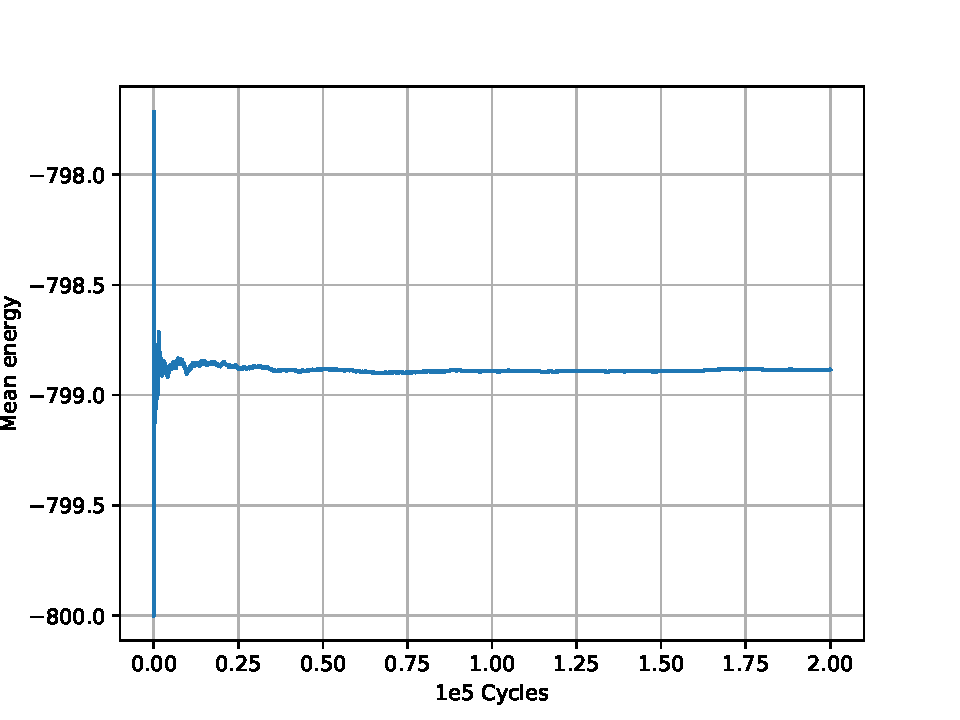
\includegraphics[scale=0.56]{../opp_c_e_10K_200000_o.pdf}
	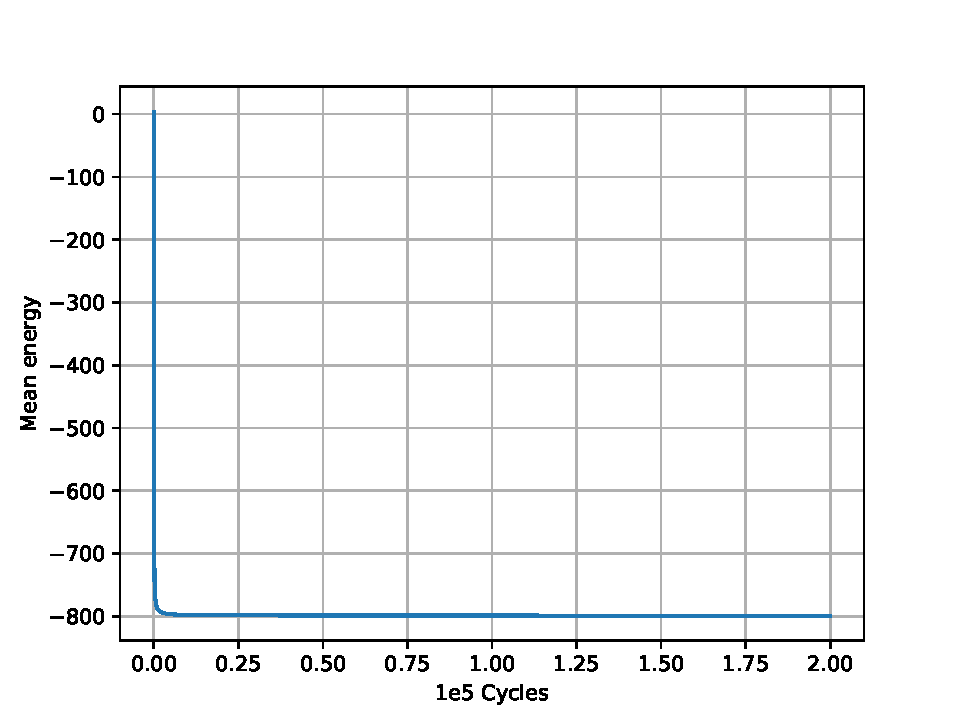
\includegraphics[scale=0.56]{../opp_c_e_10K_200000_r.pdf}
	\caption{A plot of energy at $T = 1J/k_B T$ for a ordered spin matrix on the left, and a random spin matrix on the right}
	%Label gjør det enkelt å referere til ulike bilder.
	\label{c_e_1}
\end{figure}
\begin{figure}[!htb]
	\centering 
	%Scale angir størrelsen på bildet. Bildefilen må ligge i samme mappe som tex-filen. 
	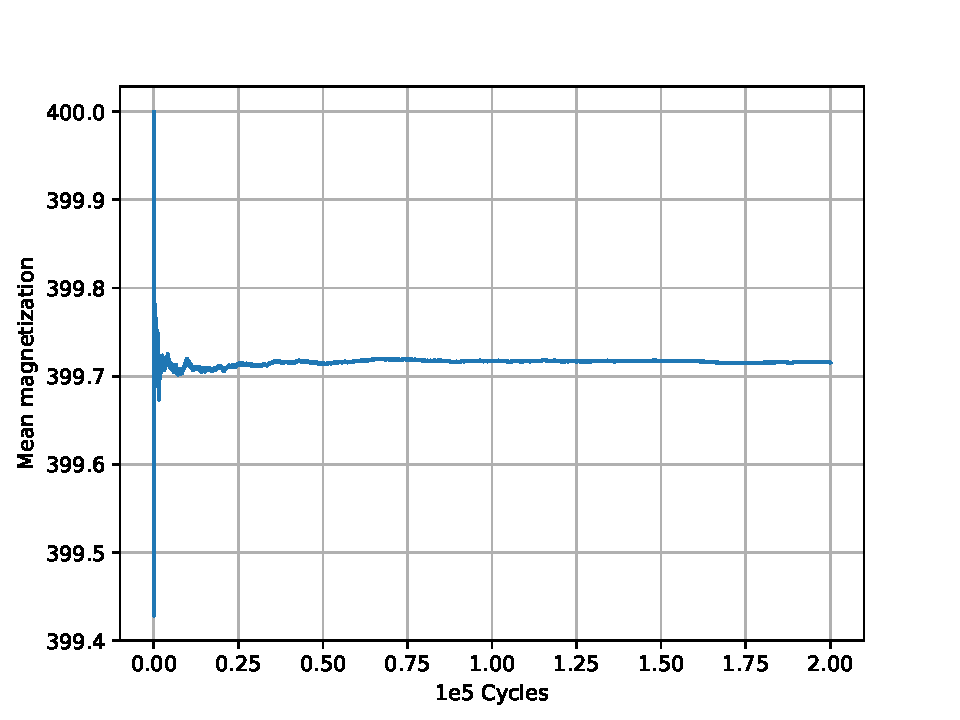
\includegraphics[scale=0.56]{../opp_c_m_10K_200000_o.pdf}
	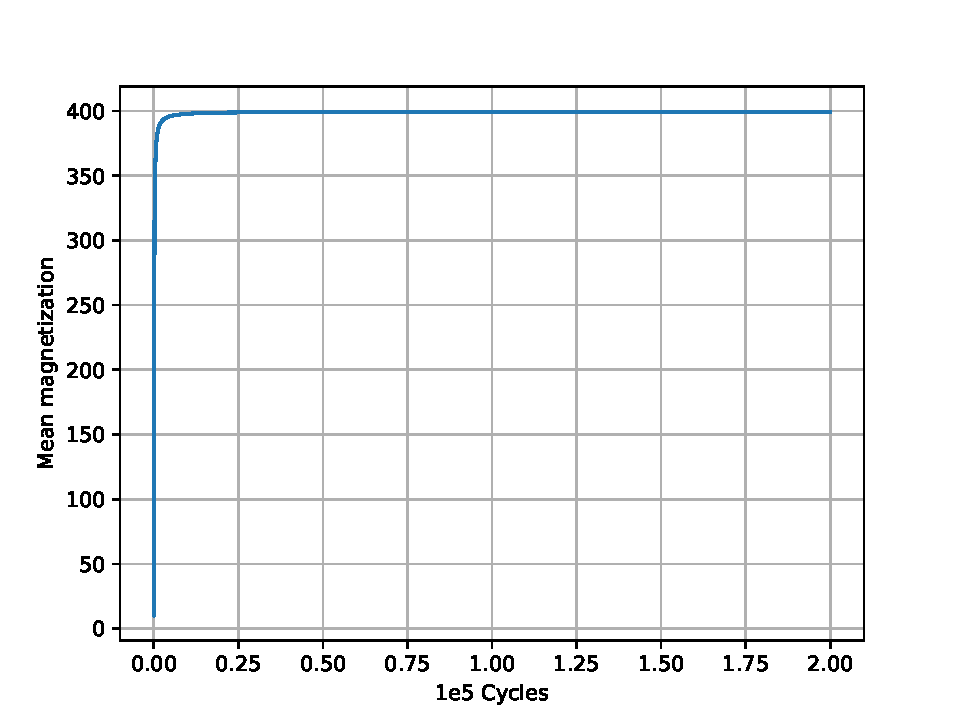
\includegraphics[scale=0.56]{../opp_c_m_10K_200000_r.pdf}
	\caption{A plot of magnetization at $T = 1J/k_B T$ for a ordered spin matrix on the left, and a random spin matrix on the right}
	%Label gjør det enkelt å referere til ulike bilder.
	\label{c_m_1}
\end{figure}
\begin{figure}[!htb]
	\centering 
	%Scale angir størrelsen på bildet. Bildefilen må ligge i samme mappe som tex-filen. 
	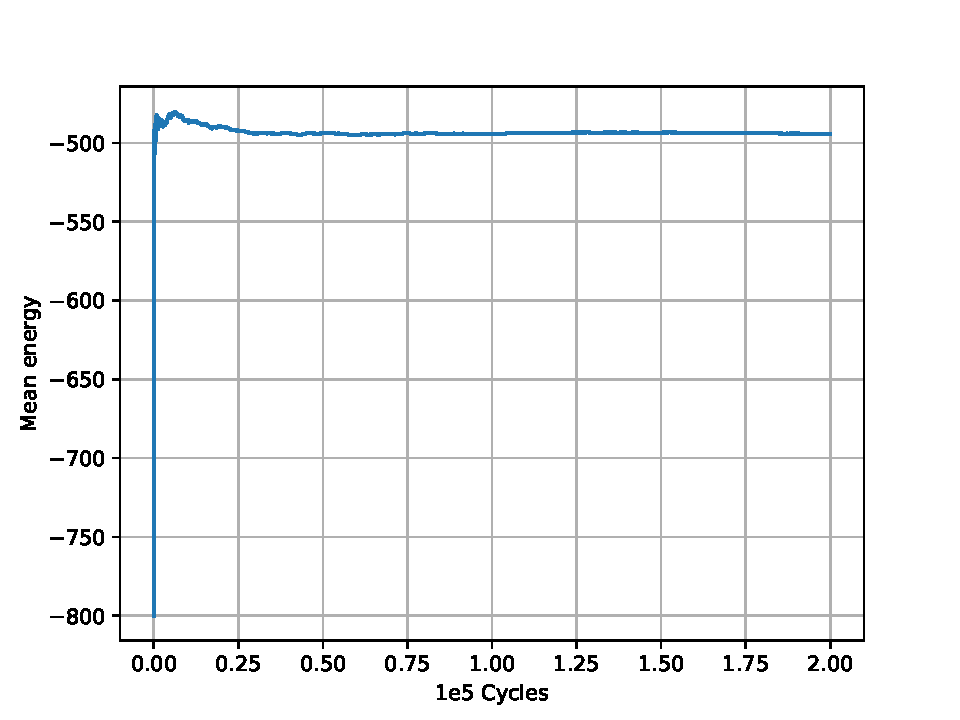
\includegraphics[scale=0.56]{../opp_c_e_24K_200000_o.pdf}
	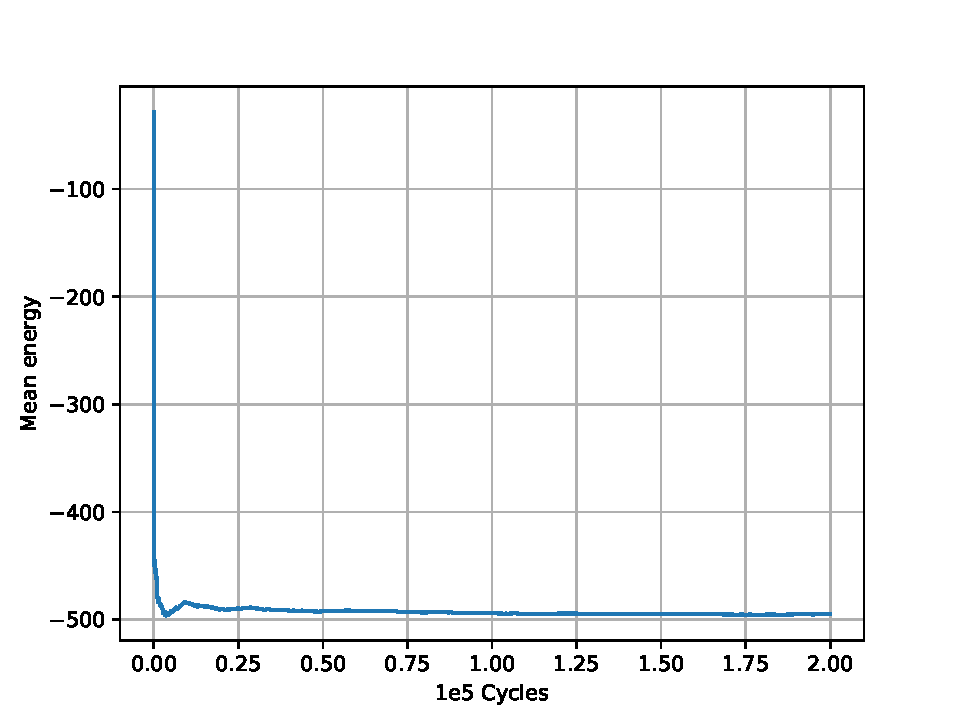
\includegraphics[scale=0.56]{../opp_c_e_24K_200000_r.pdf}
	\caption{A plot of energy at $T = 2.4 J/k_B T$ for a ordered spin matrix on the left, and a random spin matrix on the right}
	%Label gjør det enkelt å referere til ulike bilder.
	\label{c_e_2.4}
\end{figure}
\begin{figure}[!htb]
	\centering 
	%Scale angir størrelsen på bildet. Bildefilen må ligge i samme mappe som tex-filen. 
	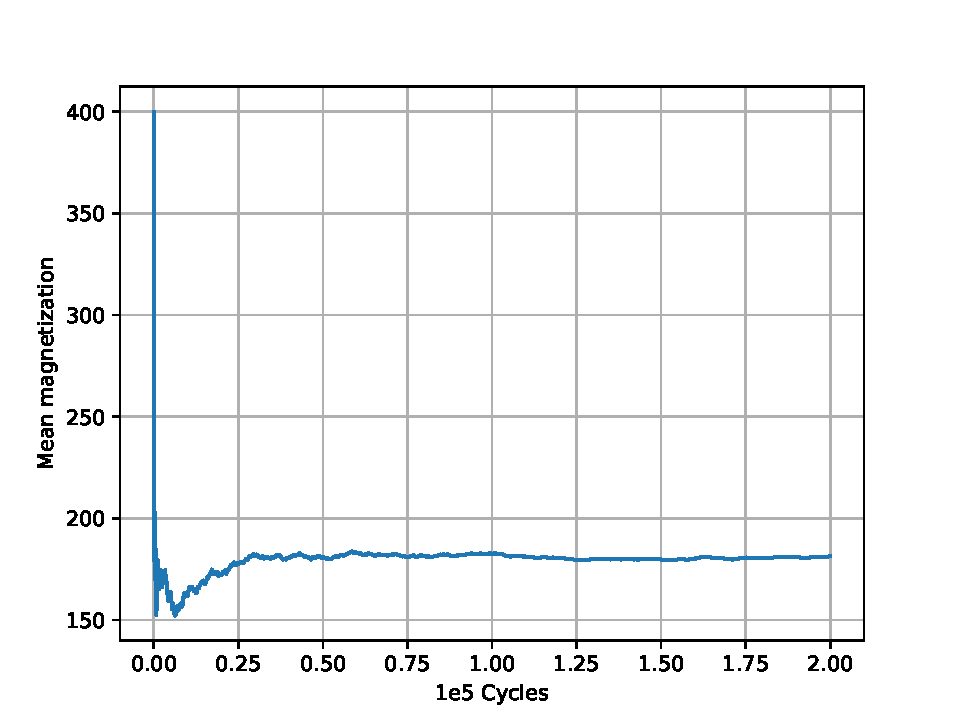
\includegraphics[scale=0.56]{../opp_c_m_24K_200000_o.pdf}
	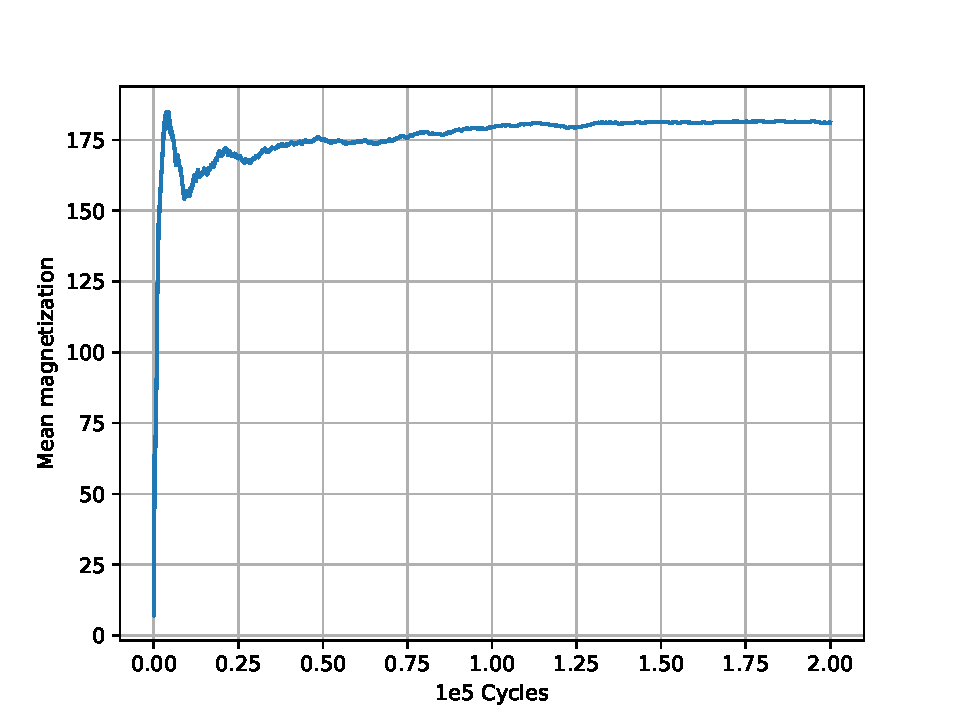
\includegraphics[scale=0.56]{../opp_c_m_24K_200000_r.pdf}
	\caption{A plot of magnetization at $T = 2.4 J/k_B T$ for a ordered spin matrix on the left, and a random spin matrix on the right}
	%Label gjør det enkelt å referere til ulike bilder.
	\label{c_m_2.4}
\end{figure}


\begin{figure}[!htb]
	\centering 
	%Scale angir størrelsen på bildet. Bildefilen må ligge i samme mappe som tex-filen. 
	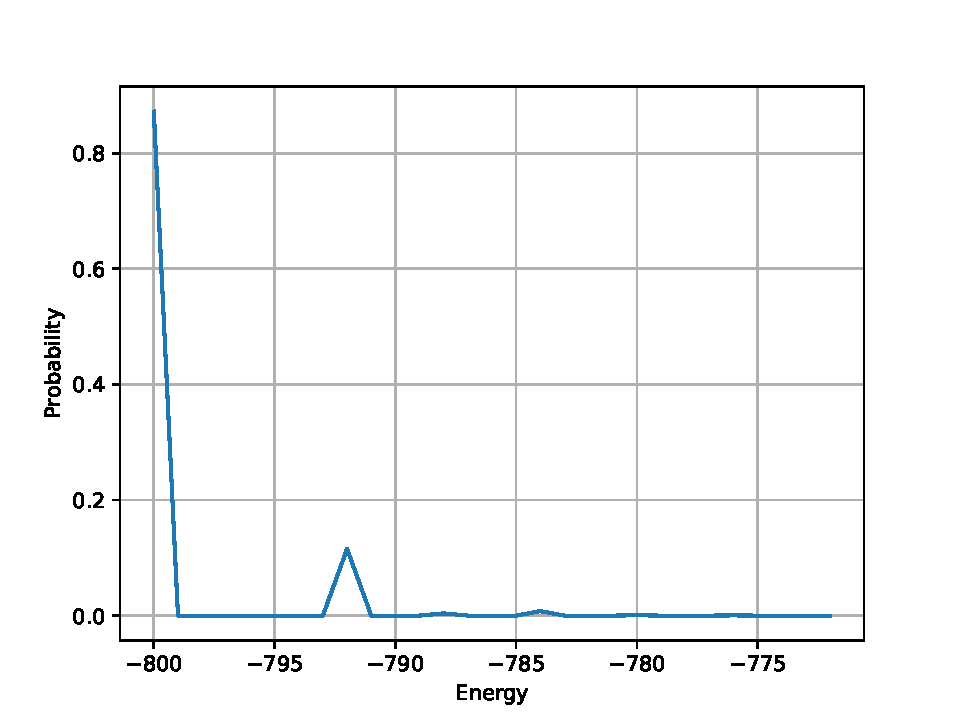
\includegraphics[scale=0.56]{../opp_d_100000_10K.pdf}
	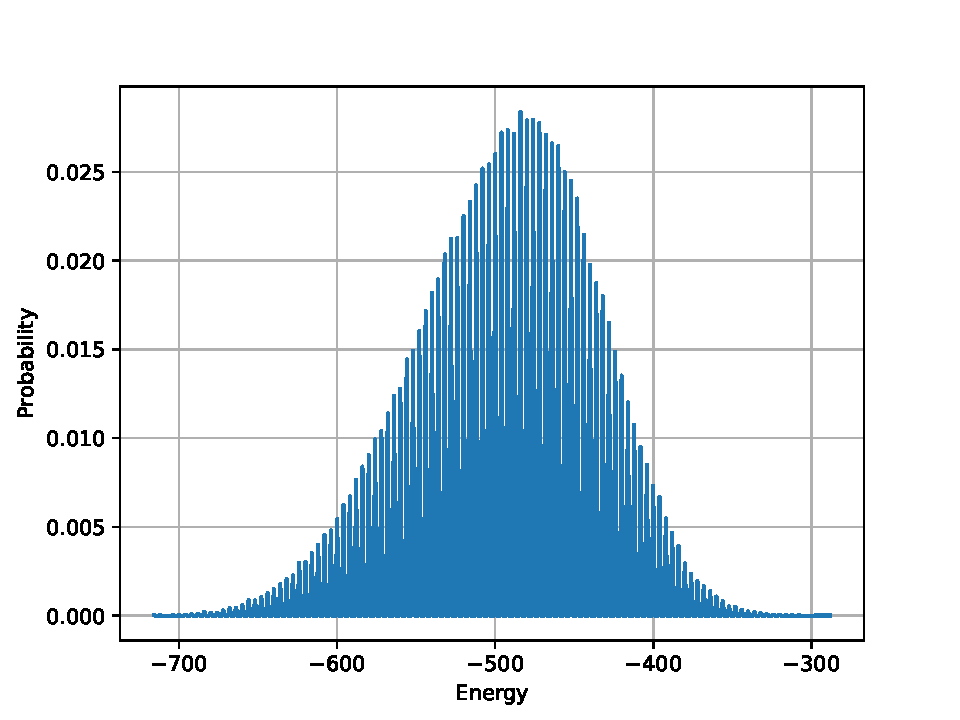
\includegraphics[scale=0.56]{../opp_d_200000_240K.pdf}
	\caption{A plot of the probability of $s$ having a certain energy after the steady state situation has been reached}
	%Label gjør det enkelt å referere til ulike bilder.
	\label{d}
\end{figure}

\subsection{Phase transitions}

A plot of the mean energy and a plot the mean magnetization against temperature can be seen in figure \ref{e}, and a plot of the specific heat and a plot the susceptibility against temperature can be seen in figure \ref{e0}.

\begin{figure}[!htb]
	\centering 
	%Scale angir størrelsen på bildet. Bildefilen må ligge i samme mappe som tex-filen. 
	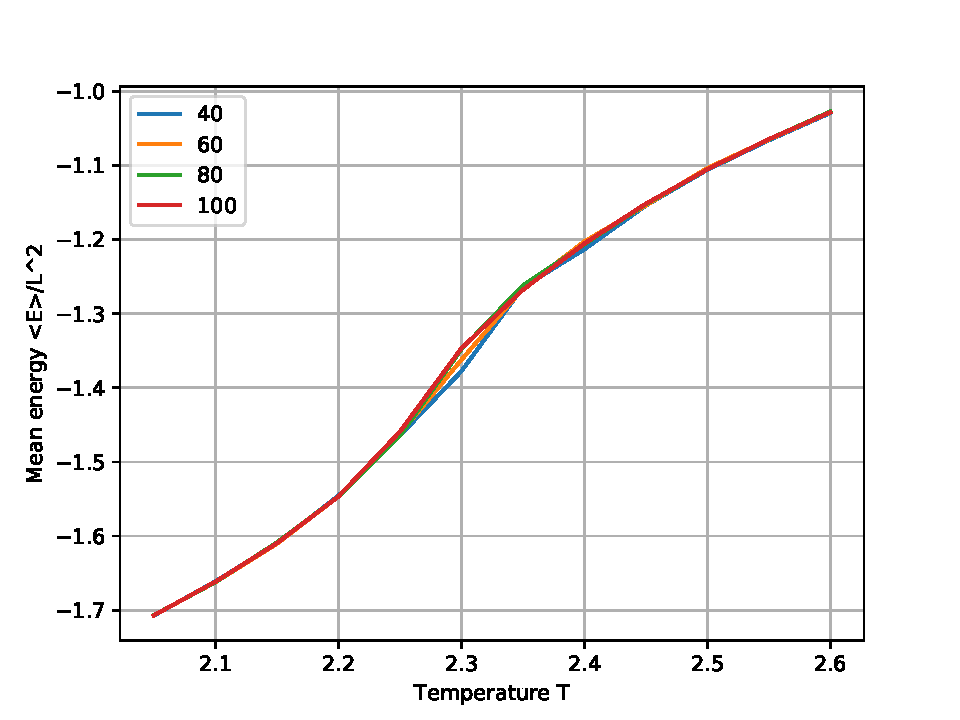
\includegraphics[scale=0.56]{../opp_e_me0.pdf}
	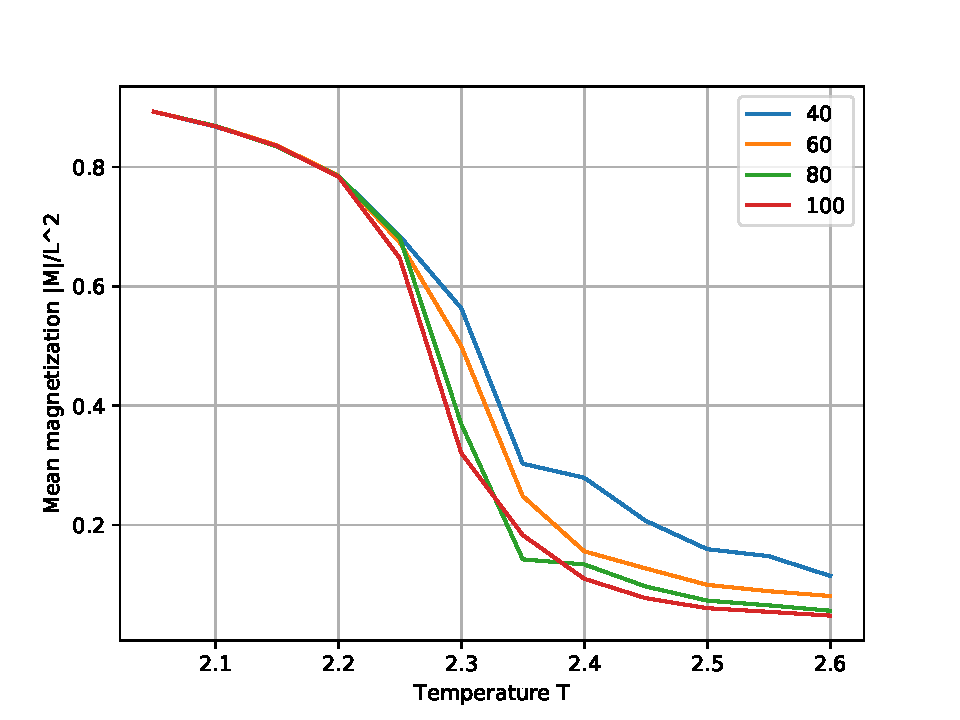
\includegraphics[scale=0.56]{../opp_e_mm0.pdf}
	\caption{The plot of the mean energy on the left, and the mean magnetization on the right, against temperature, with $L = 40, L = 60, L = 80$ and $L = 100$}
	%Label gjør det enkelt å referere til ulike bilder.
	\label{e}
\end{figure}
\begin{figure}[!htb]
	\centering 
	%Scale angir størrelsen på bildet. Bildefilen må ligge i samme mappe som tex-filen. 
	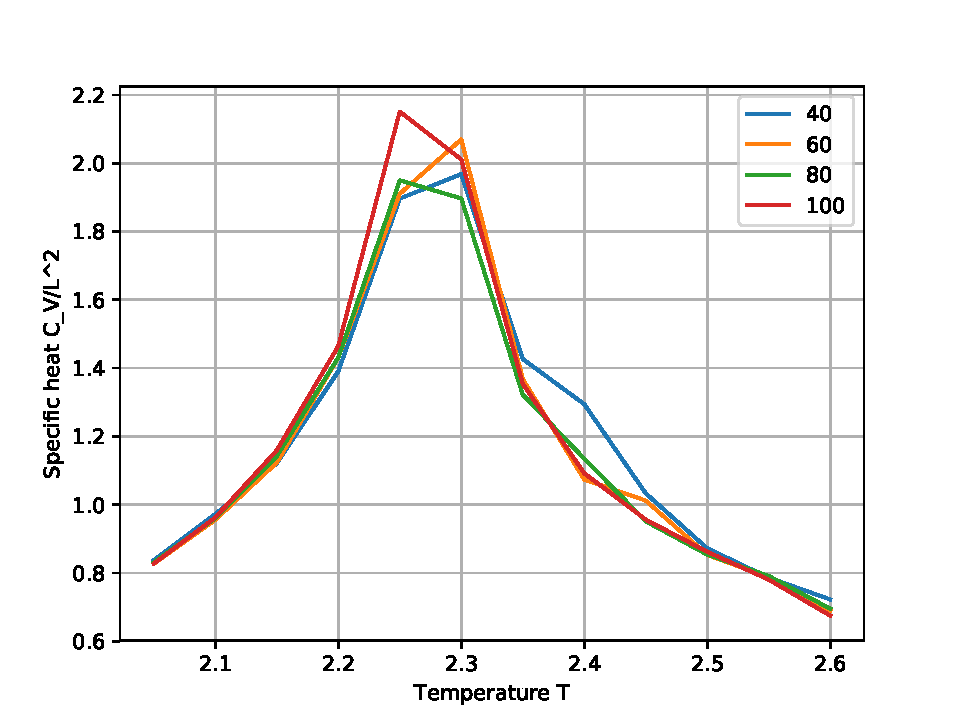
\includegraphics[scale=0.56]{../opp_e_cv0.pdf}
	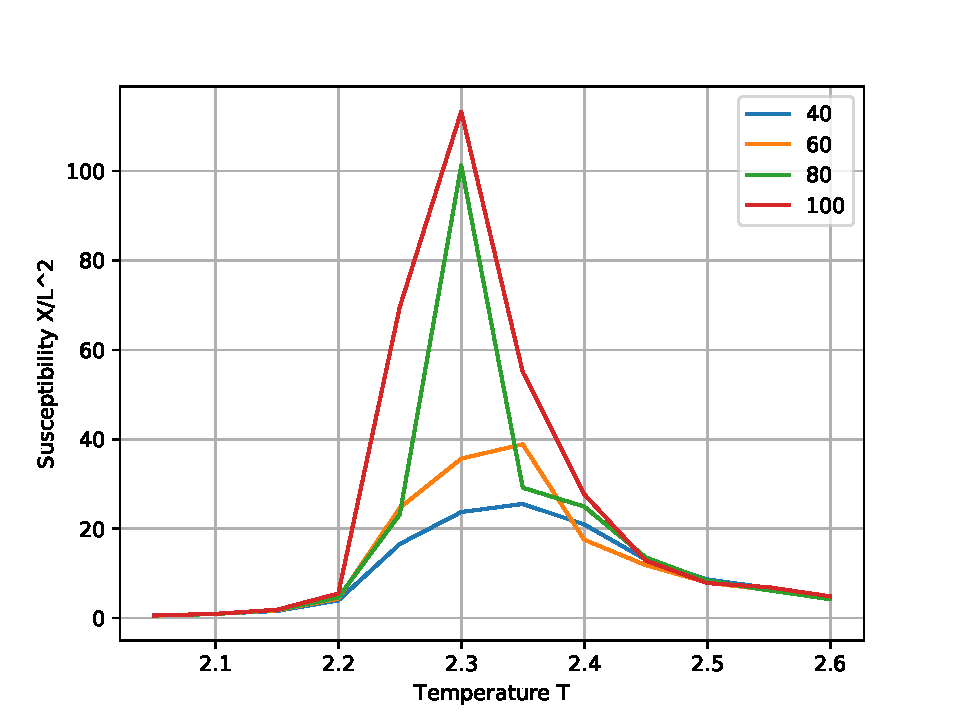
\includegraphics[scale=0.56]{../opp_e_xi0.pdf}
	\caption{The plot of the specific heat on the left, and the susceptibility on the right, against temperature, with $L = 40, L = 60, L = 80$ and $L = 100$}
	%Label gjør det enkelt å referere til ulike bilder.
	\label{e0}
\end{figure}

\section{DISCUSSION}

Looking at table \ref{tab:oppb} we can see that the discrepancy between the analytical and numerical values are quite low for $E$ and $|M|$, but about 3 orders of magnitude larger for $C_V$ and $\chi$. The discrepancies when we have $10^4$ cycles are quite large, and this is likely too few cycles. At $10^5$ cycles the discrepancies are still a bit large high, but by at $10^6$ cycles we have a very good agreement between the values, so the best number of cycles probably lies between these. Interestingly the discrepancy increases when we go to $10^7$ cycles. What is likely happening here is that the system has stabilised somewhere before reaching $10^6$ cycles, and we are not going to receive a more accurate result, but when giong to $10^7$ cycles the result becomes less accurate due to round of errors or overflow. 

If we observe figure \ref{c_e_1} to \ref{c_m_2.4} we can see that the time it takes for the system to stabilize varies depending on the temperature and whereter the spin matrix is ordered or random. The system stabilises quite quickly in figure \ref{c_e_1}, \ref{c_m_1} and \ref{c_e_2.4}, somewhere before $0.75\cdot 10^5$ cycles. Figure \ref{c_m_2.4} looks to have stabilized by the end of the plot, but is also relatively stable after $10^5$ cycles, so going forward we assumed the steady state situation would have been reached by that point. Also of note is that the values converges to a certain value based on the temperature, but not based of whereter the spin matrix is ordered or random. At $T=1$ the ordered values starts close to this value, meaning that the steady state situation here is close to a ordered spin matrix. The same is not true at $T=2.4$.

If we look at figure \ref{d} we can see that the probability distribution for the energy is quite different at $T=1$ and at $T=2.4$. At $T=1$ most of the probability lays at $E=-800$, with some variation up to $E=-772$. This indicates that the steady state situation at $T=1$ is extremely stable, with little variance in the energy. Surprisingly enough we do not get a Gaussian distribution, as we would expect from a case of randomness. This could be because the most likely energy is also the lowest possible energy, and a Gaussian distribution would therefore be impossible. The fact that the most likely value is $E=-800$ is consistent with figure \ref{c_e_1}. 
At $T=2.4$ the probability distribution is closer to a Gaussian distribution. The energy goes from $E=-716$ to $E=-288$, which means the variance is about 15 times larger than at $T=1$. This indicates that steady state situation at $T=2.4$ is more unstable. The most likely value of $E$ is around $-500$, which is consistent with figure \ref{c_e_2.4}.

If we observe figure \ref{e} we can see that the mean energy against temperature forms a s-curve. There's a good agreement between the graphs regardless of the value of $L$, except for around $T=2.3$ where they split up a bit.  $\langle E\rangle$ seems to approach $-1$ as $T$ increases, but might approach $0$ as $T$ increases even more. In figure \ref{c_e_1} the curve approached $\langle E\rangle=-800$, meaning $\langle E\rangle/L^2 = -2$ there. Similarly, the plot of the mean magnetization also forms a s-curve, but here there's more disagreement between the different $L$-values. At around $t=2.2$ the curves starts splitting up, with the higher $L$-values underneath the lower ones. $\langle |M|\rangle$ seems to approach $0$ as $T$ increases. In figure \ref{c_m_1} the mean magnetization approached $400$, meaning $\langle |M|\rangle/L^2$ equaled $1$. This, and the similar observations about $\langle E\rangle$, suggest that the steady state situation at $T=1$ is a ordered spin matrix, and approaches a spin matrix with a even distribution between positive and negative spins as $T$ increases. From observing figure \ref{e0} we can see that both the specific heat and the susceptibility increases exponentially at the start, but around $T=2.3$ they turn and decrease again. This is in line with figure \ref{e}, where the turning point for the s-curves seems to be around $T=2.3$. This suggest that the critical temperature $T_C$ is somewhere around that point, but a more detailed plot with a lower $\Delta T$ would be needed to make a good estimation. Interestingly there's a large discrepancy between the different values for $L$ in the plot of the susceptibility, but not for the specific heat. The reason this happens is unknown.



%\newpage
\section{APPENDICES}
All the calculations were done using the programing language Julia. The programs used can be found at:
\url{https://github.com/bendkok/FYS-3150/tree/master/Prosjekt%204}.
	
	%\section{REFERENCES}
	\begin{thebibliography}{9}
		\bibitem{lecture notes}
		Computational Physics, Lecture Notes Fall 2015, Morten Hjort-Jensen p. 419-424
	\end{thebibliography}
	
	
	
	
	%\begin{figure}[h!]
	%	\centering 
	%	%Scale angir størrelsen på bildet. Bildefilen må ligge i samme mappe som tex-filen. 
	%	\includegraphics[scale=0.7]{opp2_7.pdf}
	%	\caption{A plot of the entropy}
	%	%Label gjør det enkelt å referere til ulike bilder.
	%	\label{2.7}
	%\end{figure}
	
	
	
	
	
	
	
	
	
	
	
	
	
	
	
	
	
	
	
	
	
	
\end{document}




